\documentclass{standalone}
\usepackage{tikz}
\usetikzlibrary{arrows}

\begin{document}
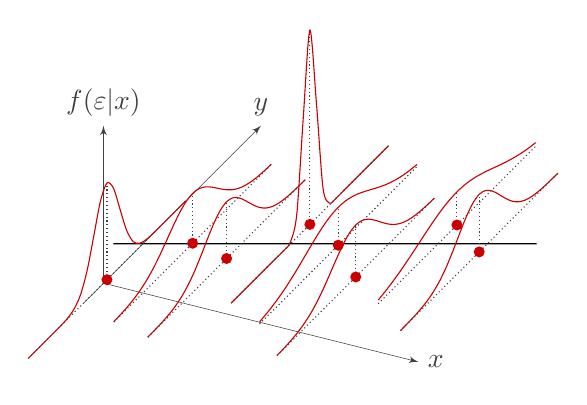
\begin{tikzpicture}[z=.5cm, x={(1cm,-.25cm)}]
%Axis 
\draw[darkgray, very thin, -latex'] (0,0,0) -- (4,0,0) node[right]{$x$};
\draw[darkgray, very thin, -latex'] (0,0,0) -- (0,2,0) node[above]{$f(\varepsilon|x)$};
\draw[darkgray, very thin, -latex'] (0,0,-.5) -- (0,0,4) node[above]{$y$};
% Regression equation
\draw (-.3,0,.85) -- (4,0,3);   
\pgfmathsetseed{3}              % Seed fixed for replicabilty
\foreach \xval in {0,.5,...,3.5}{
  \pgfmathsetmacro{\eps}{rand};  % Save the residual (to be able to use its value prior to update)
  \pgfmathsetmacro{\sigma}{rnd}; % Save the variance (to be able to use its value prior to update)
  \draw[red!80!black] plot[domain=-2:2,smooth] (\xval, {0.3989/\sigma*exp((-1/2)*((\x/\sigma)^2))}, {\x + 1 + \xval/2+\eps}); % Standard normal 
  \draw[darkgray, densely dotted] (\xval,0, 1+\xval/2+\eps) ++(0,0,-2) -- ++(0,0,4);      %Horizontal help line
  \draw[darkgray, densely dotted] (\xval,0, 1+\xval/2+\eps) -- ++(0,{0.3989/\sigma))},0); %Vertical help line
  \fill[red!80!black] (\xval, 0, 1+\xval/2+\eps) circle (.7mm);                            % y=1+x/2
}
\end{tikzpicture}
\end{document}
